\documentclass[]{beamer}
\mode<presentation>

\usepackage[utf8]{inputenc}
\usepackage[portuges]{babel}
\usepackage[T1]{fontenc}
\usepackage{multicol} % split into columns
\usepackage[]{csquotes}

\setbeamertemplate{footline}[page number]
\setbeamercovered{transparent}
\beamertemplatenavigationsymbolsempty

\author[Dmitry]{Dmitry Nix \\ \texttt{@dmitrynix}}

\title{Biologia e Matemática na Genética}
\institute{UFPI}
\date{29 de Novembro de 2014}

\begin{document}
  \begin{frame}
    \titlepage
  \end{frame}

  %\begin{frame}{Índice}
    %\tableofcontents
  %\end{frame}

  \begin{frame}{Eucarioto e Procarioto}
    \begin{center}
      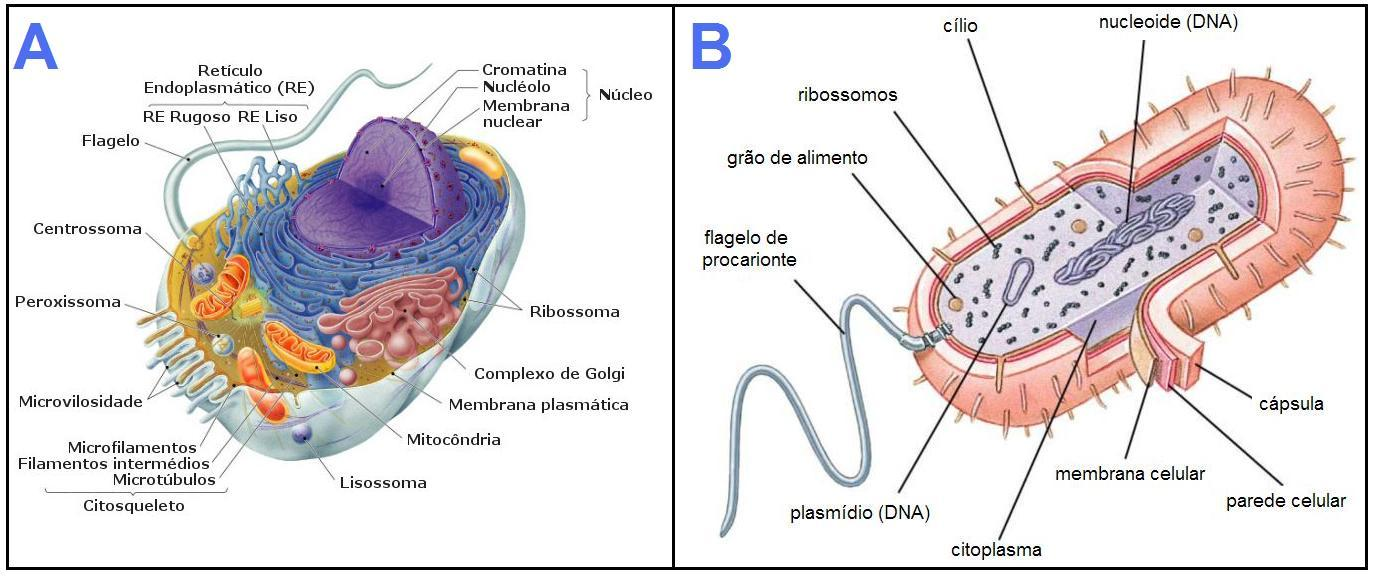
\includegraphics[width=11cm]{images/eucarioto-procarioto.png}
    \end{center}
  \end{frame}

  \begin{frame}{DNA e RNA}
    \begin{center}
      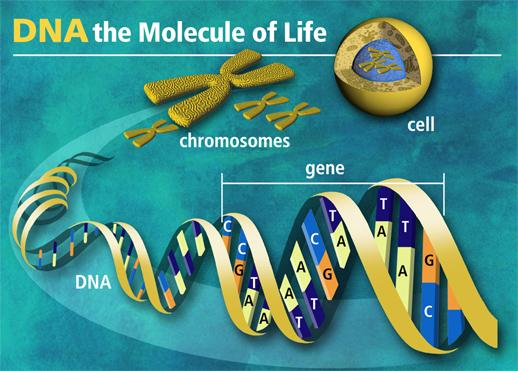
\includegraphics[width=10cm]{images/dna-e-rna-1.png}
    \end{center}
  \end{frame}

  \begin{frame}{DNA e RNA}
    \begin{center}
      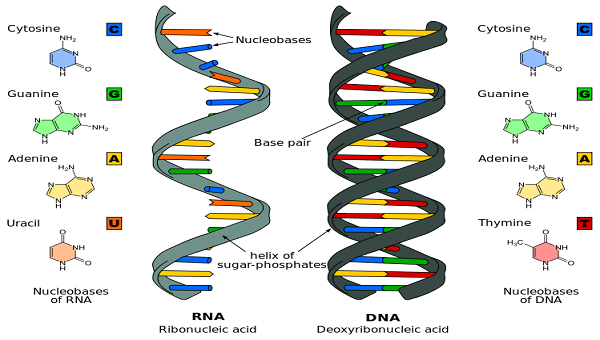
\includegraphics[width=11cm]{images/dna-e-rna.png}
    \end{center}
  \end{frame}

  \begin{frame}{Proteínas}
    \begin{center}
      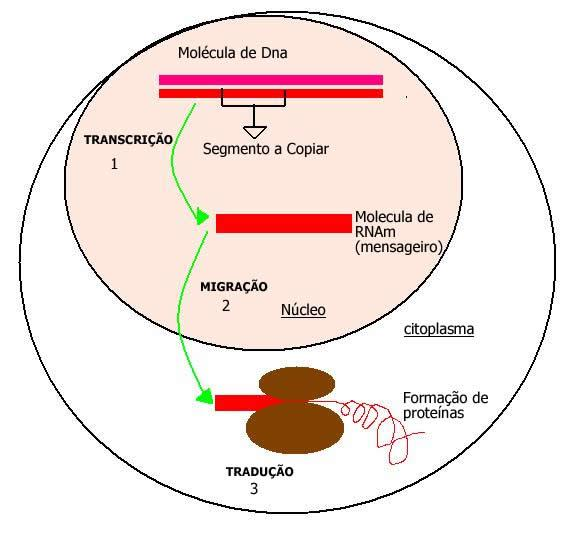
\includegraphics[width=8cm]{images/proteinas-1.png}
    \end{center}
  \end{frame}

  \begin{frame}{Proteínas}
    \begin{center}
      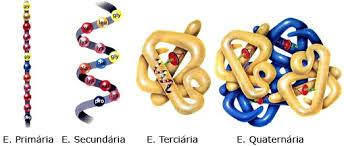
\includegraphics[width=8cm]{images/proteinas-2.png}
    \end{center}
  \end{frame}

  \begin{frame}{Cromossomos}
    \begin{center}
      \begin{multicols}{2}
        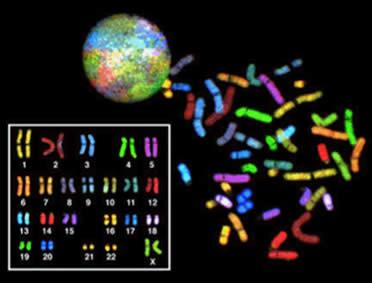
\includegraphics[width=5cm]{images/cromossomos-1.png}
        \columnbreak

        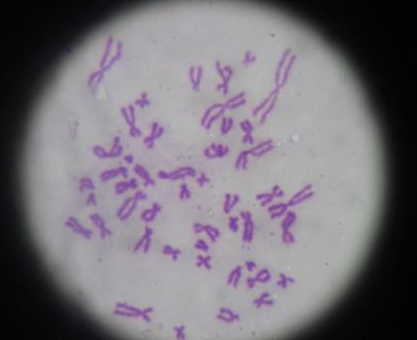
\includegraphics[width=6cm]{images/cromossomos-2.png}
      \end{multicols}
    \end{center}
  \end{frame}

  \begin{frame}{Divisão celular}
    \begin{center}
      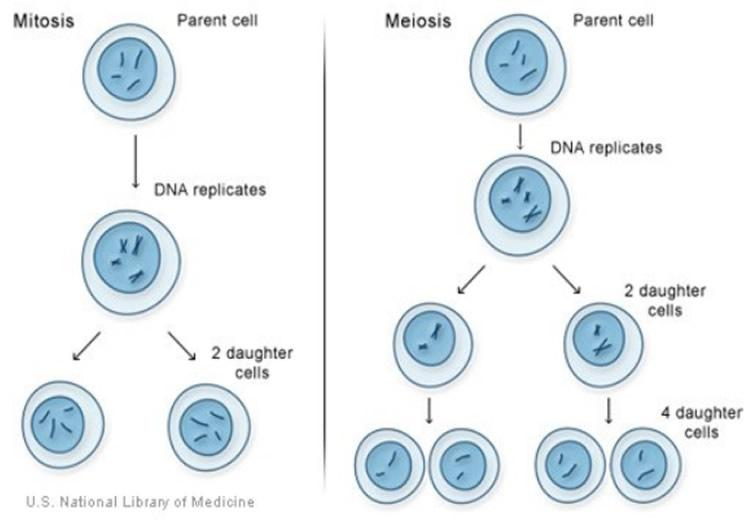
\includegraphics[width=9cm]{images/divisao-celular.png}
    \end{center}
  \end{frame}

  \begin{frame}{A importância de Mendel para a Genética}
    \begin{center}
      A maioria dos biólogos acreditava que a hereditariedade baseava-se na transmissão de entidades matérias dos pais para os filhos.
    \end{center}
  \end{frame}

  \begin{frame}{A ervilha como material experimental}
    \begin{center}
      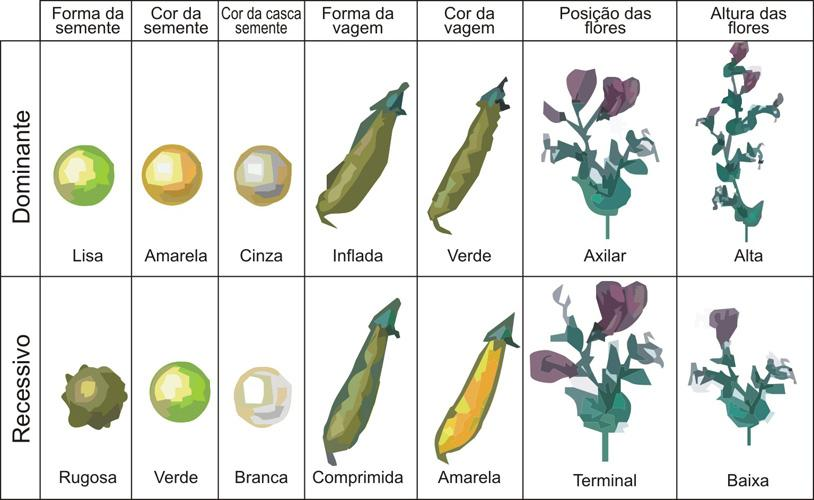
\includegraphics[width=8cm]{images/ervilha.png}

      \hspace{0.5cm}

      Mendel iniciou seus trabalhos com 34 variedades diferentes de ervilha.
    \end{center}
  \end{frame}

  \begin{frame}{1º lei de Mendel: Lei da segregação dos fatores genéticos}
    \begin{center}
      Cada característica é determinada por dois fatores que se separam na formação dos gametas, onde ocorrem em dose simples.

      \hspace{0.5cm}

      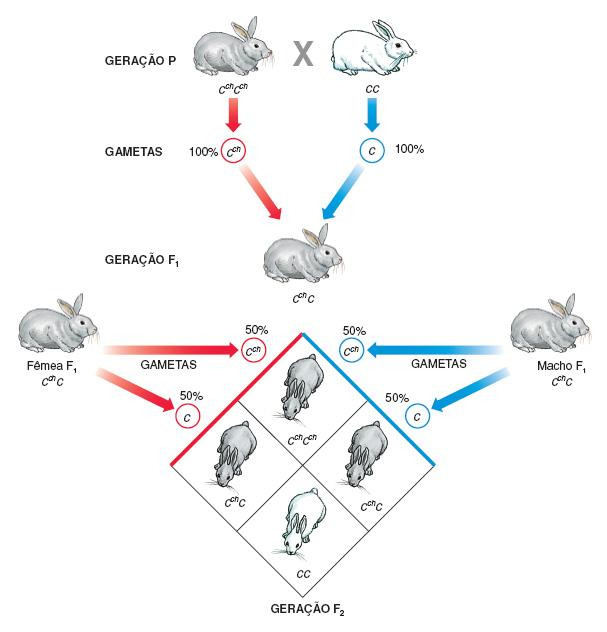
\includegraphics[width=6cm]{images/coelhos.png}
    \end{center}
  \end{frame}

  \begin{frame}{2º Lei de Mendel: Lei da segregação independente}
    \begin{center}
      Os fatores para duas ou mais características segregam-se no híbrido, distribuindo-se independentemente para os gametas, onde se combinam ao acaso.

      \hspace{0.5cm}

      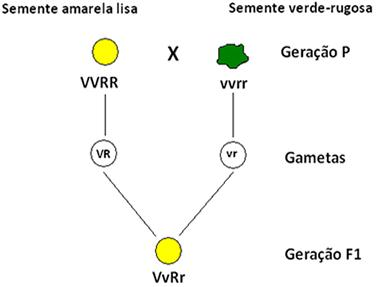
\includegraphics[width=5cm]{images/image1.png}
    \end{center}
  \end{frame}

  \begin{frame}{2º Lei de Mendel: Lei da segregação independente}
    \begin{center}
        Mendel sempre observou, em F2, a proporção fenotípica 9:3:3:1, consequência da segregação independente ocorrida no duplo-heterozigoto, que origina quatro tipos de gameta.

        \hspace{0.5cm}

        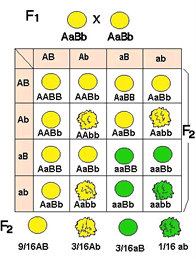
\includegraphics[width=4cm]{images/proporcao1-edited}
    \end{center}
  \end{frame}

  \begin{frame}{Sistema ABO de grupos sanguíneos na espécie humana}
    \begin{center}
      \begin{multicols}{2}
        \begin{itemize}
          \item Karl Landsteiner verificou a incompatibilidade sanguínea entre certas pessoas
            \footnote{
              A incompatibilidade deve-se a uma reação imunológica presente no plasma sanguíneo
            };
          \item O sistema ABO compreende dois tipos de aglutinogênios (A e B) e dois tipos de aglutininas (anti-A e anti-B)
        \end{itemize}

        \columnbreak
        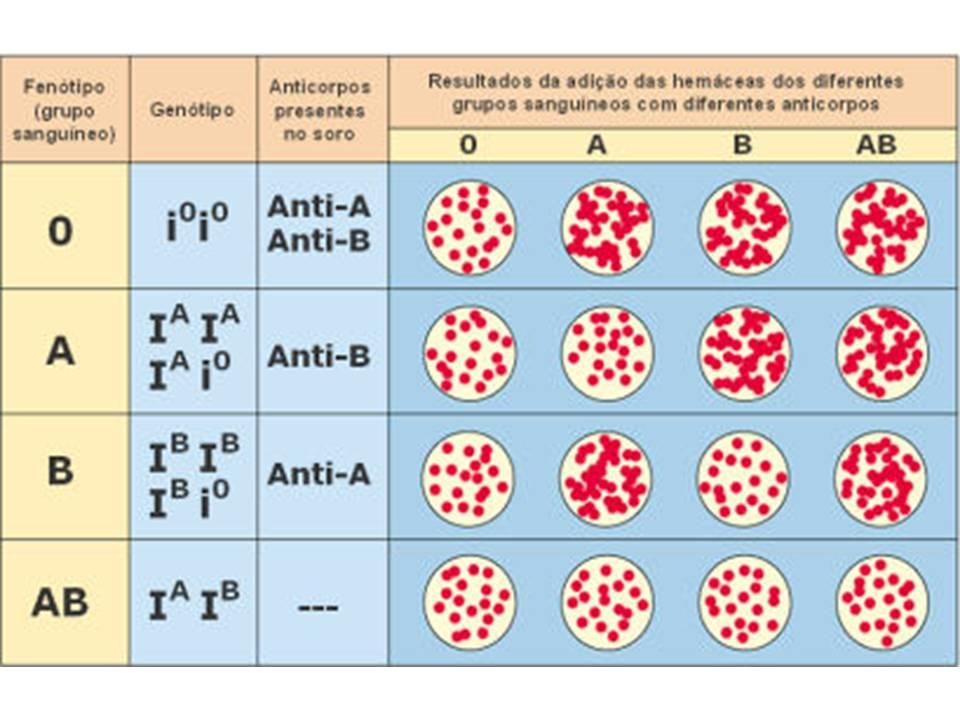
\includegraphics[width=6cm]{images/abo.png}
      \end{multicols}
    \end{center}
  \end{frame}

  \begin{frame}{Determinação do Sexo: Sistema XY}
    \begin{center}
      \begin{itemize}
        \item A determinação do sexo depende em última análise, da ação de genes específicos que atuam no desenvolvimento do novo ser, fazendo com que ele se torne macho ou fêmea.
        \item As fêmeas têm um par de cromossomos homólogos, os machos tem um par de crmossomos distintos.
        \begin{itemize}
          \item Cromossomo X - Presente tanto em fêmeas quanto nos machos.
          \item Cromossomo Y - Presente nos machos.
        \end{itemize}
      \end{itemize}

      \hspace{0.5cm}

      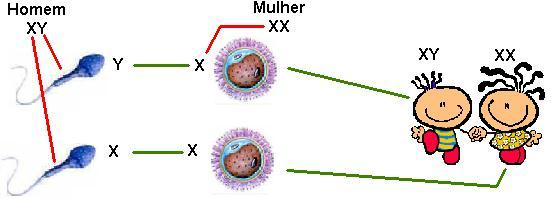
\includegraphics[width=6cm]{images/xy.png}
    \end{center}
  \end{frame}
\end{document}
